\documentclass[11pt,letterpaper]{article}
\usepackage[lmargin=1in,rmargin=1in,tmargin=1in,bmargin=1in]{geometry}
\usepackage{../style/homework}
\usepackage{../style/commands}
\setbool{quotetype}{true} % True: Side; False: Under
\setbool{hideans}{true} % Student: True; Instructor: False

% -------------------
% Content
% -------------------
\begin{document}

\homework{15: Due 12/12}{The linear programming was---and is---perhaps the single most important real-life problem.}{Keith Devin}

% Problem 1
\problem{10} Consider the function $z= 5x_1 - 6x_2$ on the region $\mathcal{R}$ shown below. Does $z$ have a maximum or minimum value on $\mathcal{R}$? Explain. If the function has a maximum or minimum value on $\mathcal{R}$, find the maximum and minimum value. 
	\[
	\fbox{
	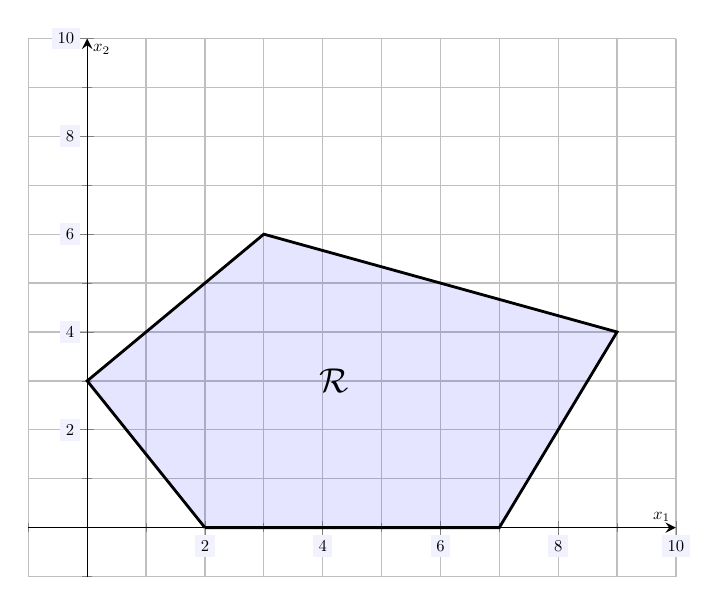
\begin{tikzpicture}[scale=1.2,every node/.style={scale=0.5}]
	\begin{axis}[
	grid=both,
	axis lines=middle,
	ticklabel style={fill=blue!5!white},
	xmin= -1, xmax=10,
	ymin= -1, ymax=10,
	xtick={0,2,4,6,8,10},
	ytick={0,2,4,6,8,10},
	minor tick = {-1,0,1,...,10},
	xlabel=\(x_1\),ylabel=\(x_2\),
	]
	\draw[line width=0.01cm,fill= blue,opacity=0.1] (2,0) -- (0,3) -- (3,6) -- (9,4) -- (7,0) -- (2,0);
	\draw[line width=0.03cm] (2,0) -- (0,3) -- (3,6) -- (9,4) -- (7,0) -- (2,0);
	\node at (4.2,3) {\huge$\mathcal{R}$};
	\end{axis}
	\end{tikzpicture}
	}
	\]



\newpage



% Problem 2
\problem{10} Consider the function $z= -3x_1 + 8x_2$ on the region $\mathcal{R}$ shown below. Does $z$ have a maximum or minimum value on $\mathcal{R}$? Explain. If the function has a maximum or minimum value on $\mathcal{R}$, find the maximum and minimum value. 
	\[
	\fbox{
	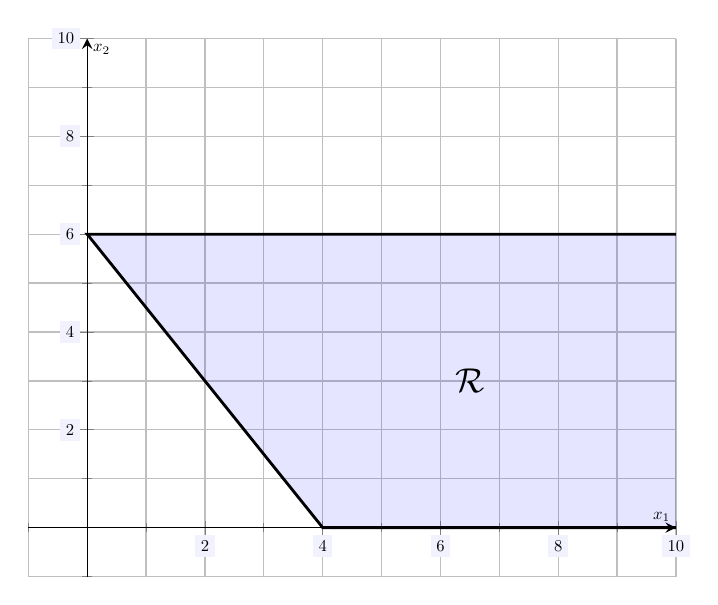
\begin{tikzpicture}[scale=1.2,every node/.style={scale=0.5}]
	\begin{axis}[
	grid=both,
	axis lines=middle,
	ticklabel style={fill=blue!5!white},
	xmin= -1, xmax=10,
	ymin= -1, ymax=10,
	xtick={0,2,4,6,8,10},
	ytick={0,2,4,6,8,10},
	minor tick = {-1,0,1,...,10},
	xlabel=\(x_1\),ylabel=\(x_2\),
	]
	
	\draw[line width=0.01cm,fill= blue,opacity=0.1] (4,0) -- (2,3) -- (0,6) -- (10,6) -- (10,0) -- (4,0);
	\draw[line width=0.03cm] (10,0) -- (4,0) -- (2,3) -- (0,6) -- (10,6);
	\node at (6.5,3) {\huge$\mathcal{R}$};
	\end{axis}
	\end{tikzpicture}
	}
	\]



\newpage



% Problem 3
\problem{10} Consider the function $z= x_1 - 9x_2$ on the region $\mathcal{R}$ shown below. Does $z$ have a maximum or minimum value on $\mathcal{R}$? Explain. If the function has a maximum or minimum value on $\mathcal{R}$, find the maximum and minimum value. 
	\[
	\fbox{
	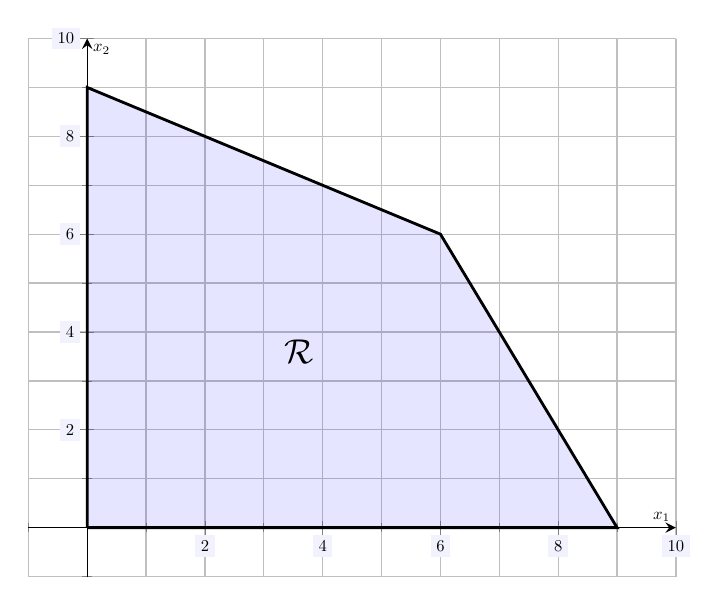
\begin{tikzpicture}[scale=1.2,every node/.style={scale=0.5}]
	\begin{axis}[
	grid=both,
	axis lines=middle,
	ticklabel style={fill=blue!5!white},
	xmin= -1, xmax=10,
	ymin= -1, ymax=10,
	xtick={0,2,4,6,8,10},
	ytick={0,2,4,6,8,10},
	minor tick = {-1,0,1,...,10},
	xlabel=\(x_1\),ylabel=\(x_2\),
	]
	\draw[line width=0.01cm,fill= blue,opacity=0.1] (0,0) -- (0,9) -- (6,6) -- (9,0) -- (0,0);
	\draw[line width=0.03cm] (0,0) -- (0,9) -- (6,6) -- (9,0) -- (0,0);
	\node at (3.6,3.6) {\huge$\mathcal{R}$};
	\end{axis}
	\end{tikzpicture}
	}
	\]



\newpage



% Problem 4
\problem{10} Find the dual problem for the minimization problem shown below.
	\[
	\begin{gathered}
	\min w= 4y_1 + 6y_2 - 9y_3 \\
	\begin{cases}
	7y_1 + 3y_2 + 8y_3 \geq 37 \\
	4y_1 - y_2 + 5y_3 \geq 55 \\
	y_1 - y_2 + 3y_3 \leq 18 \\
	y_1, y_2, y_3 \geq 0
	\end{cases}
	\end{gathered}
	\]


\end{document}